%package list
\documentclass{article}
\usepackage[top=3cm, bottom=3cm, outer=3cm, inner=3cm]{geometry}
\usepackage{multicol}
\usepackage{graphicx}
\usepackage{url}
%\usepackage{cite}
\usepackage{hyperref}
\usepackage{array}
%\usepackage{multicol}
\newcolumntype{x}[1]{>{\centering\arraybackslash\hspace{0pt}}p{#1}}
\usepackage{natbib}
\usepackage{pdfpages}
\usepackage{multirow}
\usepackage[normalem]{ulem}
\useunder{\uline}{\ul}{}
\usepackage{svg}
\usepackage{xcolor}
\usepackage{listings}
\lstdefinestyle{ascii-tree}{
    literate={├}{|}1 {─}{--}1 {└}{+}1 
  }
\lstset{basicstyle=\ttfamily,
  showstringspaces=false,
  commentstyle=\color{red},
  keywordstyle=\color{blue}
}
%\usepackage{booktabs}
\usepackage{caption}
\usepackage{subcaption}
\usepackage{float}
\usepackage{array}

\newcolumntype{M}[1]{>{\centering\arraybackslash}m{#1}}
\newcolumntype{N}{@{}m{0pt}@{}}


%%%%%%%%%%%%%%%%%%%%%%%%%%%%%%%%%%%%%%%%%%%%%%%%%%%%%%%%%%%%%%%%%%%%%%%%%%%%
%%%%%%%%%%%%%%%%%%%%%%%%%%%%%%%%%%%%%%%%%%%%%%%%%%%%%%%%%%%%%%%%%%%%%%%%%%%%
\newcommand{\itemEmail}{}
\newcommand{\itemStudent}{Arce Mayhua Leonardo  Velasque Arcos Mikhail  Quispe Saavedra Dennis }
\newcommand{\itemCourse}{Programación web 2}
\newcommand{\itemCourseCode}{}
\newcommand{\itemSemester}{I}
\newcommand{\itemUniversity}{Universidad Nacional de San Agustín de Arequipa}
\newcommand{\itemFaculty}{Facultad de Ingeniería de Producción y Servicios}
\newcommand{\itemDepartment}{Departamento Académico de Ingeniería de Sistemas e Informática}
\newcommand{\itemSchool}{Escuela Profesional de Ingeniería de Sistemas}
\newcommand{\itemAcademic}{2024 - A}
\newcommand{\itemInput}{Del 3 de junio del 2024}
\newcommand{\itemOutput}{Al 9 de Junio del 2024}
\newcommand{\itemPracticeNumber}{06}
\newcommand{\itemTheme}{Aplicaicon del Django a nuestra base de datos}
%%%%%%%%%%%%%%%%%%%%%%%%%%%%%%%%%%%%%%%%%%%%%%%%%%%%%%%%%%%%%%%%%%%%%%%%%%%%
%%%%%%%%%%%%%%%%%%%%%%%%%%%%%%%%%%%%%%%%%%%%%%%%%%%%%%%%%%%%%%%%%%%%%%%%%%%%

\usepackage[english,spanish]{babel}
\usepackage[utf8]{inputenc}
\AtBeginDocument{\selectlanguage{spanish}}
\renewcommand{\figurename}{Figura}
\renewcommand{\refname}{Referencias}
\renewcommand{\tablename}{Tabla} %esto no funciona cuando se usa babel
\AtBeginDocument{%
	\renewcommand\tablename{Tabla}
}

\usepackage{fancyhdr}
\pagestyle{fancy}
\fancyhf{}
\setlength{\headheight}{30pt}
\renewcommand{\headrulewidth}{1pt}
\renewcommand{\footrulewidth}{1pt}
\fancyhead[L]{\raisebox{-0.2\height}{
\includegraphics[width=3cm]{img/logo_episunsa.png}}}
\fancyhead[C]{\fontsize{7}{7}\selectfont	\itemUniversity \\ \itemFaculty \\ \itemDepartment \\ \itemSchool \\ \textbf{\itemCourse}}
\fancyhead[R]{\raisebox{-0.2\height}{
\includegraphics[width=1.2cm]{img/logo_abet}}}
\fancyfoot[L]{Integrantes}
\fancyfoot[C]{\itemCourse}
\fancyfoot[R]{Página \thepage}

% para el codigo fuente
\usepackage{listings}
\usepackage{color, colortbl}
\definecolor{dkgreen}{rgb}{0,0.6,0}
\definecolor{gray}{rgb}{0.5,0.5,0.5}
\definecolor{mauve}{rgb}{0.58,0,0.82}
\definecolor{codebackground}{rgb}{0.95, 0.95, 0.92}
\definecolor{tablebackground}{rgb}{0.8, 0, 0}

\lstset{frame=tb,
	language=bash,
	aboveskip=3mm,
	belowskip=3mm,
	showstringspaces=false,
	columns=flexible,
	basicstyle={\small\ttfamily},
	numbers=none,
	numberstyle=\tiny\color{gray},
	keywordstyle=\color{blue},
	commentstyle=\color{dkgreen},
	stringstyle=\color{mauve},
	breaklines=true,
	breakatwhitespace=true,
	tabsize=3,
	backgroundcolor= \color{codebackground},
}

\begin{document}
	
	\vspace*{10px}
	
	\begin{center}	
		\fontsize{17}{17} \textbf{ Informe de Laboratorio \itemPracticeNumber}
	\end{center}
	\centerline{\textbf{\Large Tema: \itemTheme}}
	%\vspace*{0.5cm}	

	\begin{flushright}
		\begin{tabular}{|M{2.5cm}|N|}
			\hline 
			\rowcolor{tablebackground}
			\color{white} \textbf{Nota}  \\
			\hline 
			     \\[30pt]
			\hline 			
		\end{tabular}
	\end{flushright}	

	\begin{table}[H]
		\begin{tabular}{|x{4.7cm}|x{4.8cm}|x{4.8cm}|}
			\hline 
			\rowcolor{tablebackground}
			\color{white} \textbf{Estudiante} & \color{white}\textbf{Escuela}  & \color{white}\textbf{Asignatura}   \\
			\hline 
			{\itemStudent \par \itemEmail} & \itemSchool & {\itemCourse \par Semestre: \itemSemester \par Código: \itemCourseCode}     \\
			\hline 			
		\end{tabular}
	\end{table}		
	
	\begin{table}[H]
		\begin{tabular}{|x{4.7cm}|x{4.8cm}|x{4.8cm}|}
			\hline 
			\rowcolor{tablebackground}
			\color{white}\textbf{Laboratorio} & \color{white}\textbf{Tema}  & \color{white}\textbf{Duración}   \\
			\hline 
			\itemPracticeNumber & \itemTheme & 04 horas   \\
			\hline 
		\end{tabular}
	\end{table}
	
	\begin{table}[H]
		\begin{tabular}{|x{4.7cm}|x{4.8cm}|x{4.8cm}|}
			\hline 
			\rowcolor{tablebackground}
			\color{white}\textbf{Semestre académico} & \color{white}\textbf{Fecha de inicio}  & \color{white}\textbf{Fecha de entrega}   \\
			\hline 
			\itemAcademic & \itemInput &  \itemOutput  \\
			\hline 
		\end{tabular}
	\end{table}
	%%%%%%%%%%%%%%%%%%%%%%%%%%%%%%%%%%%%%%%%%%%%%%%%%%%%%%%%%%%%%%%%%%%%%%%%%%%%%%%%%%%%%%%%%%%%%%%%%%%%%%%%%%%%%%%%%%%%%%%%%%%%%%%%%%%%%%%%%%%%%%%%%%%%%%%%%%%%%%%%%%%%%%%%%%%%%%%%%%%%%%%%%%%%%%%%%%%%
	
	
	
	
	
	\section{INTRODUCCION}
\begin{itemize}
    \item En el siguiente informe se expondrán las actividades del laboratorio 06 del curso de Programación Web 02.
    \item La presentación de los ejercicios será de la siguiente manera:
    \item Primero: Se expondrán las partes más importantes del código. En este caso, se detallará primero nuestra problemática encontrada en la mejora del sistema del comedor universitario de la UNSA.
    \item Segundo: También se expondrá lo que se hizo dentro de Django y cómo plasmamos nuestro primer borrador de un diagrama ER para esta base de datos.
\end{itemize}

\section{Problemática a tratar y el diagrama ER (primer borrador)}
\begin{itemize}
    \item En este caso, evaluamos el sistema del comedor universitario y cómo este tiene algunas deficiencias para con el comensal, empezando con la falta de un calendario que muestre la cantidad de días que el comensal no asistió al comedor, así como las fechas en que no realizó los pagos correspondientes para una semana determinada.
    \item También se observa la falta de una pestaña o sistema de justificación donde el comensal pueda acceder fácilmente para justificar sus faltas/inasistencias y la falta de pagos realizados.
\end{itemize}

\begin{figure}[H]
			\centering
			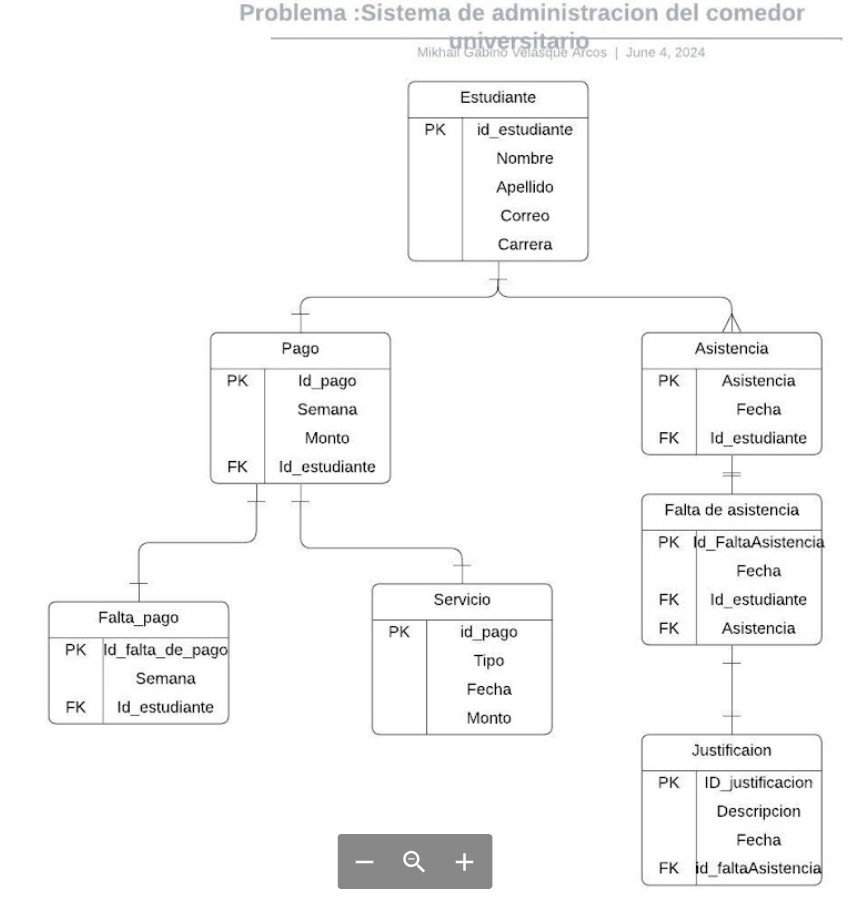
\includegraphics[scale=0.3]{img/Diagrama_ER_borrador.jpeg} 
		\end{figure}


\section{Clase Models}

En esta sección, definimos los modelos que representan las entidades del sistema del comedor universitario. Cada uno de estos modelos tiene atributos únicos y específicos, así como relaciones bien definidas entre ellos. Estos atributos permiten una gestión detallada y precisa de la información relacionada con el sistema del comedor universitario.

\subsection{Modelo Asistencia}

El modelo \texttt{Asistencia} representa la asistencia de los estudiantes al comedor universitario. Cada registro de asistencia está relacionado con un estudiante y contiene información como el estado de asistencia (registrado a través de \texttt{status}), la fecha de creación y modificación del registro (\texttt{created} y \texttt{modified}, respectivamente).

\begin{lstlisting}[language=Python, caption={Asistencia}]
from django.db import models
from .Estudiante import Estudiante

class Asistencia (models.Model):
    Estudiante = models.ForeignKey(Estudiante, on_delete=models.CASCADE)
    id_Asistencia = models.BigAutoField(primary_key=True)
    status = models.BooleanField(default=False)
    created = models.DateTimeField(editable=False, null=False, auto_now_add=True)
    modified = models.DateTimeField(null=False, auto_now=True)
\end{lstlisting}

\subsection{Modelo Estudiante}

El modelo \texttt{Estudiante} representa a los estudiantes que utilizan el comedor universitario. Contiene información básica sobre los estudiantes, como su nombre, apellido, carrera y correo electrónico. Además, se registra el estado del estudiante (\texttt{status}) y las fechas de creación y modificación del registro.

\begin{lstlisting}[language=Python, caption={Estudiante}]
from django.db import models

class Estudiante(models.Model):
    id_Estudiante = models.BigAutoField(primary_key=True)
    nombre = models.CharField(max_length=200)
    apellido = models.CharField(max_length=200)
    carrera = models.CharField(max_length=100)
    correo = models.CharField(max_length=100)
    status = models.BooleanField(default=False)
    created = models.DateTimeField(editable=False, null=False, auto_now_add=True)
    modified = models.DateTimeField(null=False, auto_now=True)
\end{lstlisting}

\subsection{Modelo FaltaAsistencia}

El modelo \texttt{FaltaAsistencia} registra las faltas de asistencia de los estudiantes al comedor universitario. Cada registro de falta de asistencia está relacionado con un registro de asistencia y contiene información sobre la fecha de la falta (\texttt{fecha}), el estado de la falta (\texttt{status}) y las fechas de creación y modificación del registro.

\begin{lstlisting}[language=Python, caption={FaltaAsistencia}]
from django.db import models
from .Asistencia import Asistencia

class FaltaAsistencia (models.Model):
    Asistencia = models.ForeignKey(Asistencia, on_delete=models.CASCADE)
    id_FaltaAsistencia = models.BigAutoField(primary_key=True)
    fecha = models.DateTimeField(editable=False, null=False, auto_now_add=True)
    status = models.BooleanField(default=False)
    created = models.DateTimeField(editable=False, null=False, auto_now_add=True)
    modified = models.DateTimeField(null=False, auto_now=True)
\end{lstlisting}

\subsection{Modelo FaltaPago}

El modelo \texttt{FaltaPago} registra las faltas de pago de los estudiantes al comedor universitario. Cada registro de falta de pago está relacionado con un registro de pago y contiene información sobre la semana correspondiente al pago (\texttt{semana}), el estado de la falta (\texttt{status}) y las fechas de creación y modificación del registro.

\begin{lstlisting}[language=Python, caption={FaltaPago}]
from django.db import models
from .Pago import Pago

class FaltaPago(models.Model):
    pago = models.ForeignKey(Pago, on_delete=models.CASCADE)
    semana = models.IntegerField(default=1)
    status = models.BooleanField(default=False)
    created = models.DateTimeField(editable=False, null=False, auto_now_add=True)
    modified = models.DateTimeField(null=False, auto_now=True)
    id_falta_pago = models.BigAutoField(primary_key=True)
\end{lstlisting}

\subsection{Modelo Justificacion}

El modelo \texttt{Justificacion} registra las justificaciones de las faltas de asistencia de los estudiantes. Cada justificación está relacionada con un registro de falta de asistencia y contiene una descripción de la justificación, la fecha de la justificación (\texttt{fecha}), el estado de la justificación (\texttt{status}) y las fechas de creación y modificación del registro.

\begin{lstlisting}[language=Python, caption={Justificacion}]

from django.db import models
from .FaltaAsistencia import FaltaAsistencia

class Justificacion(models.Model):
    FaltaAsistencia = models.ForeignKey(FaltaAsistencia, on_delete=models.CASCADE)
    id_justificacion = models.BigAutoField(primary_key=True)
    descripcion = models.TextField()
    fecha = models.DateTimeField(editable=False, null=False, auto_now_add=True)
    status = models.BooleanField(default=False)
    created = models.DateTimeField(editable=False, null=False, auto_now_add=True)
    modified = models.DateTimeField(null=False, auto_now=True)
\end{lstlisting}

\subsection{Modelo Pago}

El modelo \texttt{Pago} registra los pagos realizados por los estudiantes en el comedor universitario. Cada registro de pago está relacionado con un estudiante y contiene información sobre la semana correspondiente al pago (\texttt{semana}), el monto del pago (\texttt{monto}), el estado del pago (\texttt{status}) y las fechas de creación y modificación del registro.

\begin{lstlisting}[language=Python, caption={Pago}]
from django.db import models
from .Estudiante import Estudiante

class Pago(models.Model):
    Estudiante = models.ForeignKey(Estudiante, on_delete=models.CASCADE)
    id_pago = models.BigAutoField(primary_key=True)
    semana = models.IntegerField(default=1)
    monto = models.FloatField(default=0.0)
    status = models.BooleanField(default=False)
    created = models.DateTimeField(editable=False, null=False, auto_now_add=True)
    modified = models.DateTimeField(null=False, auto_now=True)
\end{lstlisting}

\subsection{Modelo Servicio}

El modelo \texttt{Servicio} registra los servicios proporcionados en el comedor universitario. Cada registro de servicio está relacionado con un registro de pago y contiene información sobre el tipo de servicio (\texttt{tipo}), el estado del servicio (\texttt{status}) y las fechas de creación y modificación del registro.

\begin{lstlisting}[language=Python, caption={Servicio}]
from django.db import models
from .Pago import Pago

class Servicio(models.Model):
    id_pago = models.ForeignKey(Pago, on_delete=models.CASCADE)
    id_servicio = models.BigAutoField(primary_key=True)
    tipo = models.CharField(max_length=100)
    status = models.BooleanField(default=False)
    fecha = models.DateTimeField(editable=False, null=False, auto_now_add=True)
    modified = models.DateTimeField(null=False, auto_now=True)
\end{lstlisting}

\begin{figure}[H]
    \centering
    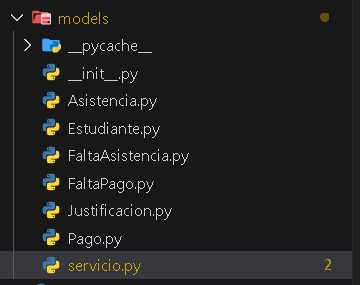
\includegraphics[scale=0.5]{img/Models.jpeg}
\end{figure}

	

	\item Cada una de estas entidades, como se puede observar, tiene atributos únicos y específicos, así como relaciones bien definidas entre ellas. Estos atributos permiten una gestión detallada y precisa de la información. Por ejemplo, el calendario de asistencia y pagos incluye atributos como la fecha, el estado de asistencia, y las fechas de modificación. Además, se establecen relaciones entre las entidades, como las que existen entre el comensal y sus registros de asistencia, y entre el comensal y sus justificativos de inasistencia o falta de pagos.
		
\item Algunos ejemplos de estos atributos son \texttt{create}, que registra la fecha de creación del registro; \texttt{status}, que indica el estado actual del registro, ya sea de asistencia o de pago; \texttt{fecha}, que especifica la fecha correspondiente a cada evento; y \texttt{modifig}, que almacena la fecha y hora de la última modificación del registro. Estos atributos y relaciones permiten una administración eficiente y detallada de todos los aspectos relacionados con el comedor universitario.


		
	
\section{Clase admin.py}
\begin{itemize}
    \item Después de haber creado cada una de las tablas dentro de los modelos, el siguiente paso es importarlas en \texttt{admin.py}. Para registrar cada modelo en el sitio de administración de Django, utilizamos la función \texttt{admin.site.register(modelo\_x)}, donde \texttt{modelo\_x} es el nombre del modelo que queremos registrar. Este proceso permite que las tablas creadas sean accesibles y administrables desde la interfaz de administración de Django, facilitando la gestión de los datos.

    \begin{itemize}
        \begin{lstlisting}[language=Python, caption={Código dentro del admin.py}]
from django.contrib import admin

from .models.Estudiante import Estudiante
from .models.Pago import Pago
from .models.servicio import servicio
from .models.FaltaPago import FaltaPago
from .models.Asistencia import Asistencia
from .models.FaltaAsistencia import FaltaAsistencia
from .models.Justificacion import Justificacion

admin.site.register(Estudiante)
admin.site.register(Pago)
admin.site.register(FaltaPago)
admin.site.register(servicio)
admin.site.register(Asistencia)
admin.site.register(FaltaAsistencia)
admin.site.register(Justificacion)
        \end{lstlisting}

        \begin{figure}[H]
            \centering
            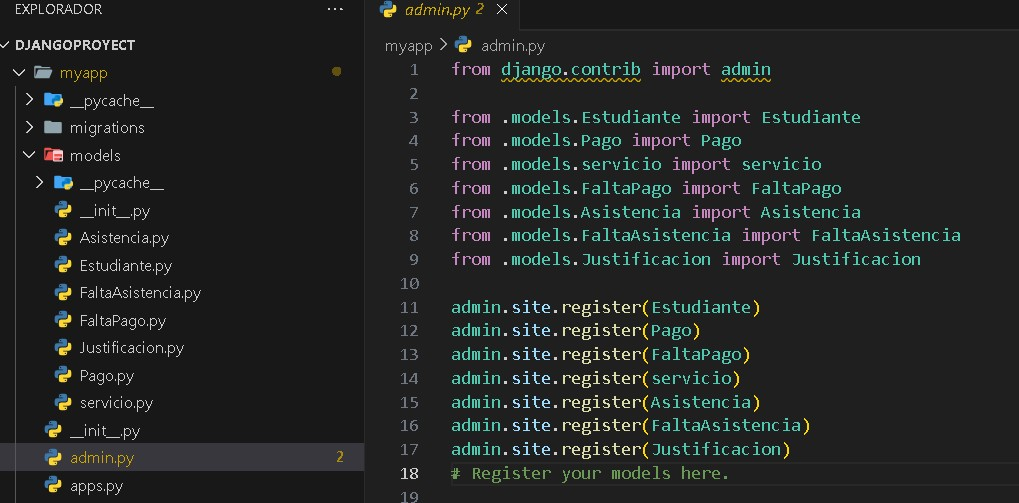
\includegraphics[scale=0.5]{img/admin.jpeg}
        \end{figure}
    \end{itemize}
\end{itemize}

     \section{Diagramas de bases de datos (ERD) desde Django}

\begin{itemize}
    \item A continuación, utilizamos una función para generar un diagrama detallado de todo lo que hemos hecho hasta ahora. Esto nos permite comparar con el primer diagrama inicial y comprender mejor el trabajo realizado, demostrando la efectividad de esta herramienta.

    \begin{lstlisting}[language=Python, caption={Comandos para la instalación y uso de Graphviz}]
1. pip install graphviz
2. pip install django-extensions
3. Agregar 'django_extensions' a INSTALLED_APPS en settings.py
4. Añadir el siguiente código a settings.py:
GRAPH_MODELS = {
    'all_applications': True,
    'graph_models': True,
}
5. pip install pyparsing pydot
6. py manage.py graph_models -a > erd.dot
7. py manage.py graph_models -a
8. py manage.py graph_models -a > erd.dot && py manage.py graph_models --pydot -a -g -o erd.png
    \end{lstlisting}

    \begin{figure}[H]
        \centering
        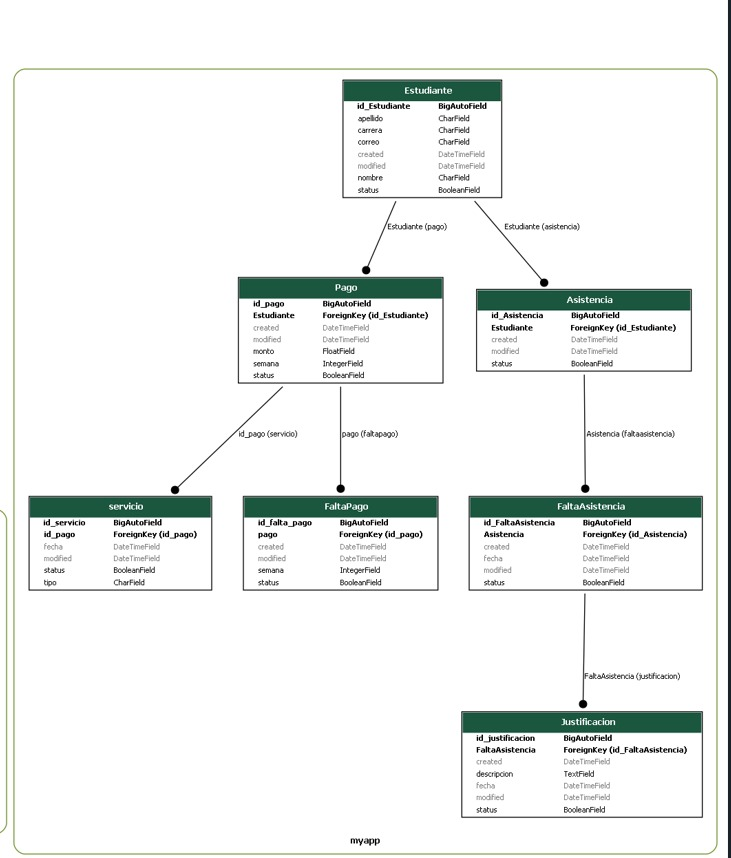
\includegraphics[scale=0.5]{img/diargamaER_FINAL.jpeg}
    \end{figure}
\end{itemize}

	
	
   \section{Ejecución del manage.py}
\begin{itemize}
    \item Para finalizar, ejecutamos el \texttt{manage.py}, lo que aplicará todos estos cambios a la base de datos y nos mostrará detalladamente todos los modelos que hemos creado, así como las configuraciones realizadas, entre otros detalles.

  \begin{lstlisting}[language=Python, caption={Comando ara el manage.py}]
 
  python manage.py createsuperuser
  
    \end{lstlisting}
    
    \item User :admin
      \item password :1234
    
    \begin{figure}[H]
        \centering
        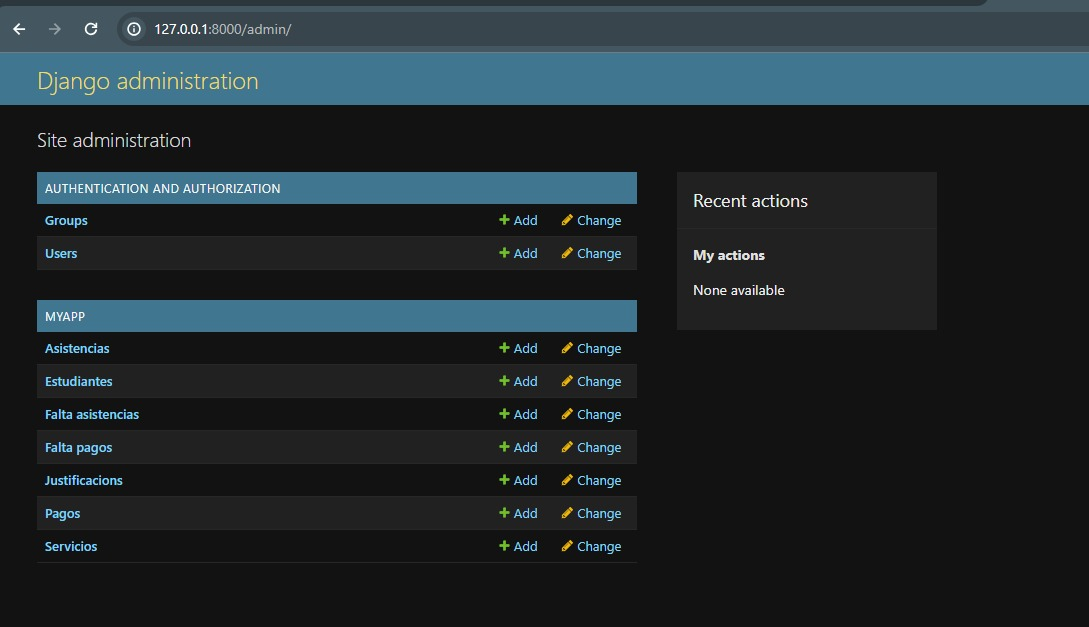
\includegraphics[scale=0.4]{img/Basedatos_final.jpeg}
    \end{figure}
\end{itemize}

	
	\section{URL GitHub }
	\begin{itemize}
		\item \url{https://github.com/mvelasquea/Pweb2_E_04.git}
	\end{itemize}
	\section{Commits }
	
	\begin{itemize}
		
		\begin{figure}[H]
			\centering
					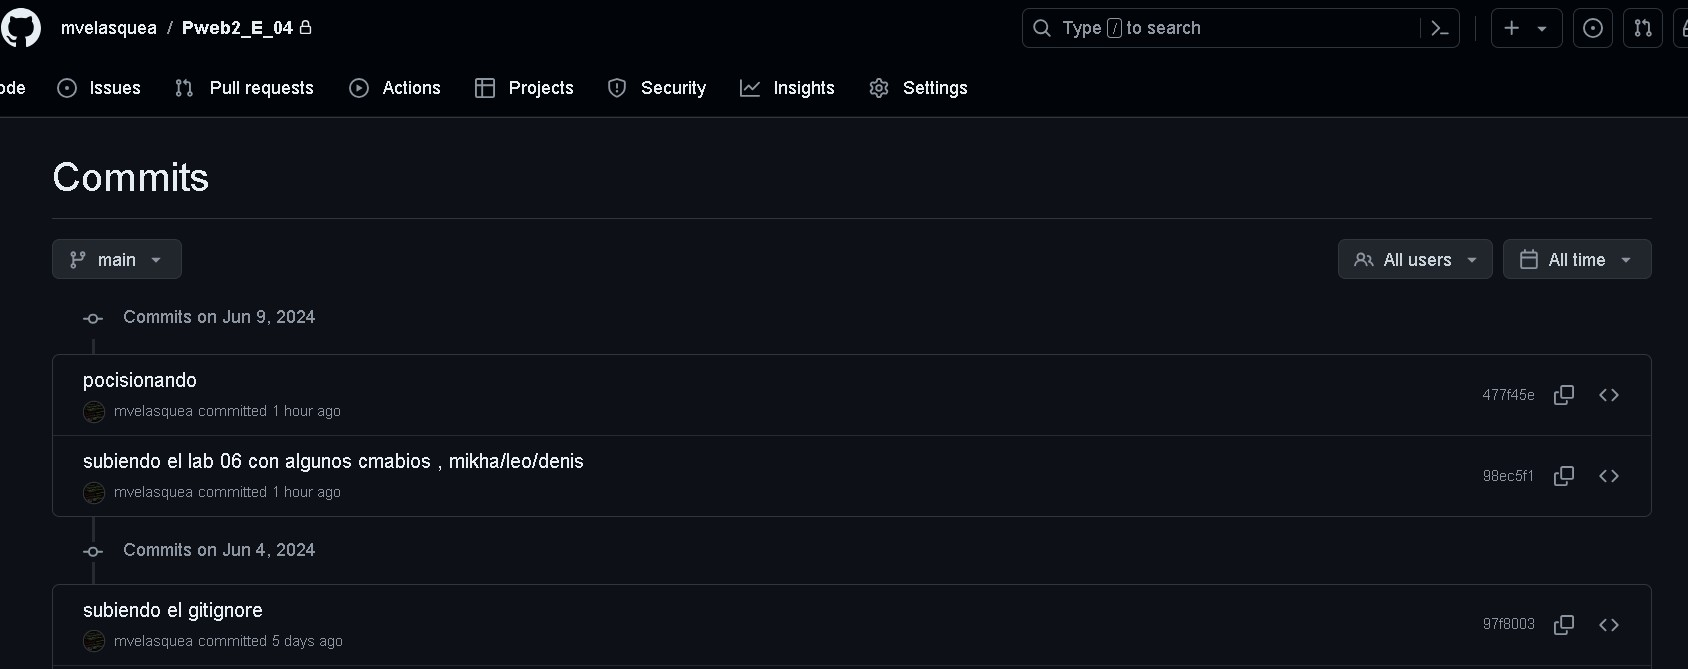
\includegraphics[scale=0.3]{img/commits.jpeg} 
		\end{figure}
	\end{itemize}
	\section{\textcolor{red}{Rúbricas}}
	
\subsection{\textcolor{red}{Rúbrica para entregable Informe}}

\begin{table}[H]
    \caption{Rúbrica para tipo de Informe}
    \setlength{\tabcolsep}{0.5em} % for the horizontal padding
    {\renewcommand{\arraystretch}{1.5}% for the vertical padding
    \begin{tabular}{|p{3cm}|p{10cm}|p{2cm}|p{2cm}|}
        \hline
        \multicolumn{2}{|c|}{\textbf{Informe}} & \textbf{Cumple} & \textbf{No cumple} \\
        \hline
        \textbf{Latex} & El informe está en formato PDF desde Latex, con un formato limpio (buena presentación) y fácil de leer. & 20 & 17 \\ 
        \hline
        \textbf{MarkDown} & El informe está en formato PDF desde MarkDown README.md, con un formato limpio (buena presentación) y fácil de leer. & 17 & 0 \\ 
        \hline
        \textbf{MS Word} & El informe está en formato PDF desde plantilla MS Word, con un formato limpio (buena presentación) y fácil de leer. & 15 & 0 \\ 
        \hline
        \textbf{Observaciones} & Por cada observación se le descontará puntos. & - & - \\
        \hline
    \end{tabular}
    }
\end{table}
	\subsection{\textcolor{red}{Rúbrica para el contenido del Informe y demostración}}
	\begin{itemize}			
		\item El alumno debe marcar o dejar en blanco en celdas de la columna \textbf{Checklist} si cumplio con el ítem correspondiente.
		\item Si un alumno supera la fecha de entrega,  su calificación será sobre la nota mínima aprobada, siempre y cuando cumpla con todos lo items.
		\item El alumno debe autocalificarse en la columna \textbf{Estudiante} de acuerdo a la siguiente tabla:
	
		\begin{table}[ht]
			\caption{Niveles de desempeño}
			\begin{center}
			\begin{tabular}{ccccc}
    			\hline
    			 & \multicolumn{4}{c}{Nivel}\\
    			\cline{1-5}
    			\textbf{Puntos} & Insatisfactorio 25\%& En Proceso 50\% & Satisfactorio 75\% & Sobresaliente 100\%\\
    			\textbf{2.0}&0.5&1.0&1.5&2.0\\
    			\textbf{4.0}&1.0&2.0&3.0&4.0\\
    		\hline
			\end{tabular}
		\end{center}
	\end{table}	
	
	\end{itemize}
	
	\begin{table}[H]
		\caption{Rúbrica para contenido del Informe y demostración}
		\setlength{\tabcolsep}{0.5em} % for the horizontal padding
		{\renewcommand{\arraystretch}{1.5}% for the vertical padding
		%\begin{center}
		\begin{tabular}{|p{2.7cm}|p{7cm}|x{1.3cm}|p{1.2cm}|p{1.5cm}|p{1.1cm}|}
			\hline
    		\multicolumn{2}{|c|}{Contenido y demostración} & Puntos & Checklist & Estudiante & Profesor\\
			\hline
			\textbf{1. GitHub} & Hay enlace URL activo del directorio para el  laboratorio hacia su repositorio GitHub con código fuente terminado y fácil de revisar. &2 &X &2 & \\ 
			\hline
			\textbf{2. Commits} &  Hay capturas de pantalla de los commits más importantes con sus explicaciones detalladas. (El profesor puede preguntar para refrendar calificación). &4 &X &4 & \\ 
			\hline 
			\textbf{3. Código fuente} &  Hay porciones de código fuente importantes con numeración y explicaciones detalladas de sus funciones. &2 &X &2 & \\ 
			\hline 
			\textbf{4. Ejecución} & Se incluyen ejecuciones/pruebas del código fuente  explicadas gradualmente. &2 &X &2 & \\ 
			\hline			
			\textbf{5. Pregunta} & Se responde con completitud a la pregunta formulada en la tarea.  (El profesor puede preguntar para refrendar calificación).  &2 &X &2 & \\ 
			\hline	
			\textbf{6. Fechas} & Las fechas de modificación del código fuente estan dentro de los plazos de fecha de entrega establecidos. &2 &X &2 & \\ 
			\hline 
			\textbf{7. Ortografía} & El documento no muestra errores ortográficos. &2 &X &1 & \\ 
			\hline 
			\textbf{8. Madurez} & El Informe muestra de manera general una evolución de la madurez del código fuente,  explicaciones puntuales pero precisas y un acabado impecable.   (El profesor puede preguntar para refrendar calificación).  &4 &X &3 & \\ 
			\hline
			\multicolumn{2}{|c|}{\textbf{Total}} &20 & &18 & \\ 
			\hline
		\end{tabular}
		%\end{center}
		%\label{tab:multicol}
		}
	\end{table}
	
\clearpage
%\clearpage
%\bibliographystyle{apalike}
%\bibliographystyle{IEEEtranN}
%\bibliography{bibliography}
			
\end{document}